%% -*- fill-column: 79; -*-

\def\currentprefix{fear-the-ear}

%\DeclareCaptionType{copyrightbox}

%% listing settings
\lstset{ %
language=Ruby,                % the language of the code
basicstyle=\footnotesize\ttfamily,       % the size of the fonts that are used for the code
escapeinside={\%*}{*)},         % if you want to add a comment within your code
morekeywords={*,...},           % if you want to add more keywords to
}

%% \title{Fear the EAR: Discovering and Mitigating \\
%%   Execution After Redirect Vulnerabilities}

%% \numberofauthors{1}

%% \author{
%% \alignauthor
%% Adam Doup\'e, Bryce Boe, Christopher Kruegel, and Giovanni Vigna\\
%% \affaddr{University of California, Santa Barbara}
%% \email{\{adoupe, bboe, chris, vigna\}@cs.ucsb.edu}
%% }

%% \maketitle
%% \begin{abstract}

%%   The complexity of modern web applications makes it difficult for
%%   developers to fully understand the security implications of their code.
%%   Attackers exploit the resulting security vulnerabilities to gain
%%   unauthorized access to the web application environment. Previous research
%%   into web application vulnerabilities has mostly focused on input
%%   validation flaws, such as cross site scripting and SQL injection, while
%%   logic flaws have received comparably less attention.

%%   In this paper, we present a comprehensive study of a relatively unknown
%%   logic flaw in web applications, which we call Execution After Redirect,
%%   or EAR. A web application developer can introduce an EAR by calling a
%%   redirect method under the assumption that execution will halt. A
%%   vulnerability occurs when server-side execution continues after the
%%   developer's intended halting point, which can lead to broken/insufficient
%%   access controls and information leakage. We start with an analysis of how
%%   susceptible applications written in nine web frameworks are to EAR
%%   vulnerabilities. We then discuss the results from the EAR challenge
%%   contained within the 2010 International Capture the Flag Competition.
%%   Finally, we present an open-source, white-box, static analysis tool to
%%   detect EARs in Ruby on Rails web applications. This tool found 3,944 EAR
%%   instances in 18,127 open-source applications. Finally, we describe an
%%   approach to prevent EARs in web frameworks.

%% \end{abstract}

%% \category{D.2.5}{Testing and Debugging}{}

%% \terms{Security}

%% \keywords{static analysis, web applications, execution after redirect}

\section{Introduction}
An increasing number of services are being offered on-line. For
example, banking, shopping, socializing, reading the news, and
enjoying entertainment are all available on the web. The increasing amount
of sensitive data stored by web applications has
attracted the attention of cyber-criminals, who break into systems to
steal valuable information such as passwords, credit card numbers,
social security numbers, and bank account credentials.

Attackers use a variety of vulnerabilities to exploit web applications. In
2008, Albert Gonzalez was accused and later convicted of stealing 40
million credit and debit cards from major corporate retailers, by writing
SQL injection attacks~\cite{gonzalez08:indictment,ortiz10:outcome}. Another
common vulnerability, cross-site scripting (XSS), is the second
highest-ranked entry on the OWASP top ten security risks for web
applications, behind injection attacks like SQL
injection~\cite{owasptopten}. Thus, SQL injection and XSS have received a
large amount of attention by the security community. Other popular web
application vulnerabilities include cross site request forgery
(XSRF)~\cite{barth08:csrf}, HTTP parameter pollution
(HPP)~\cite{carettoni09:hpp,balduzzi11:hpp}, HTTP response
splitting~\cite{klein04:http-response-splitting}, and
clickjacking~\cite{hansen08:clickjacking,balduzzi10:clickjacking}. 
\\

\noindent{}In this paper, we present an in-depth study of a little-known
real-world web application logic flaw; one we are calling Execution
After Redirect (EAR). An EAR occurs because of a developer's
misunderstanding of how the web application framework operates. In the
normal workflow of a web application, a user sends a request to the web
application. The web application receives this request, performs some
server-side processing, and returns an HTTP response. Part of the HTTP
response can be a notification that the client (a web browser) should look
elsewhere for the requested resource. In this case, the web application
sets the HTTP response code to \texttt{301}, \texttt{302},
\texttt{303}, or \texttt{307}, and adds a \texttt{Location}
header~\cite{fielding99:http11statuscode}. These response codes instruct
the browser to look for the resource originally requested at a new URL
specified by the web application in the HTTP \texttt{Location}
header~\cite{fielding99:http11location}. This process is known as
redirection\footnote{In this paper, we consider only HTTP server-side
  redirection. Other forms of redirection, executed on the client, exist
  such as JavaScript redirect or HTML meta refresh.}; the web application
redirects the user to another resource.

Intuitively, one assumes that a redirect should end execution of the
server side code; the reason is that the browser immediately sends a
request for the new location as soon as the redirection response is
received, and it does not process the rest of the web application's output. Some
web frameworks, however, do not halt execution on a redirect. This can
lead to EAR vulnerabilities.
 
Specifically, an EAR can be introduced when a web application developer
writes code that issues an HTTP redirect under the assumption that the
redirect will automatically halt execution of the web application.
Depending on the framework, execution can continue after the call to the
redirect function, potentially violating the security properties of the web
application.

We define \emph{halt-on-redirect} as a web framework behavior where
server-side code execution halts on a redirect, thus preventing EARs.
Unfortunately, some languages make halt-on-redirect difficult to implement,
for instance, by not supporting a \texttt{goto}-type statement. Therefore,
web frameworks differ in supporting halt-on-redirect behavior. This
difference in redirect method semantics can increase the developer's
confusion when developing applications in different frameworks.

In this paper, we present a comprehensive study of Execution After Redirect
vulnerabilities: we provide an overview of EARs and classify EARs into
different types. We also analyze nine web application frameworks'
susceptibility to EARs, specifying their redirect semantics, as well as
detailing what exactly makes them vulnerable to EARs. Moreover, we develop a
novel static analysis algorithm to detect EARs, which we implemented in an
open-source tool to analyze Ruby on Rails web applications. Finally, we
discovered hundreds of vulnerabilities in open-source Ruby on Rails web
applications, with a very low false positive rate.

In summary, this paper provides the following contributions:

\begin{itemize}

\item We categorize EARs and provide an analysis of nine frameworks'
  susceptibility to various types of EARs.

\item We discuss the results from the EAR challenge contained within our 2010
  International Capture the Flag Competition.

\item We present an algorithm to statically detect EARs in Ruby on
  Rails applications.

\item We run our white-box tool on 18,127 open-source Ruby on
  Rails applications, which found 3,944 EARs.

\end{itemize}

\section{Overview of EARs}
\locallabel{overview}

An Execution After Redirect vulnerability is a logic flaw in web
applications that results from a developer's misunderstanding of the
semantics of redirection. Very often this misunderstanding is caused by the
web framework used by the developer\footnote{ This misunderstanding was
  confirmed by a developer who responded to us when we notified him of an
  EAR in his code, who said, ``I wasn't aware at all of this problem
  because I thought ruby on rails will always end any execution after a
  redirect.'' This example shows that developers do not always understand
  how their web framework handles redirects.}. In particular, developers
typically assume that the web application will halt after calling a
function of the web framework that performs a redirect. Certain web
frameworks, however, do not halt execution on a redirect, and instead,
execute all the code that follows the redirect operation. The web browser
perpetuates this misunderstanding, as it obediently performs the redirect,
thus falsely indicating that the code is correct. As a result, when the
developer tests the web application using the browser, the observed
behavior seems in line with the intentions of the developer, and,
consequently, the application is assumed to be correct.

Note that an EAR is not a code injection vulnerability; an attacker
cannot execute arbitrary code, only code already present after the
redirect. An EAR is also different from XSS and
SQL injection vulnerabilities; it is not an input validation flaw, but rather a
mismatch between the developer's intentions and the actual
implementation.

\begin{lstlisting}[language=Ruby, caption=Example of an 
    Execution After Redirect vulnerability in Ruby on Rails.,
    label=\currentprefix:code:simple-ear, float,]
class TopicsController < ApplicationController 
 def update 
  @topic = Topic.find(params[:id])  
  if not current_user.is_admin?  
    redirect_to("/")
  end  
  @topic.update_attributes(params[:topic])  
  flash[:notice] = "Topic updated!"  
 end  
end 
\end{lstlisting}



As an example, consider the EAR vulnerability in the Ruby on Rails code
shown in Listing~\localref{code:simple-ear}. The code appears to redirect the
current user to ``/'' if she is not an administrator (Line~5), and, if she
is an administrator, \texttt{@topic} will be updated with the parameters
sent by the user in the \texttt{params} variable (Line~7). The code does
not execute in this way, because Ruby on Rails does not support
halt-on-redirect behavior. Thus, \emph{any} user, not only the
administrator, can update the topic, violating the intended authorization
and compromising the security of the web application.

The simple way to fix Listing~\localref{code:simple-ear} is to add a
\texttt{return} after the \texttt{redirect\_to} call on Line~5. This will
cause the \texttt{update} method to terminate after the redirect, thus, no
additional code will be executed. Adding a return after all redirects is a
good best practice, however, it is insufficient to prevent all EARs.
Listing~\localref{code:complex-ear} depicts an example of an EAR that cannot be
prevented by adding a return after a redirect. Here, the
\texttt{redirect\_to} on Line~4 is followed by a \texttt{return}, so there
is no EAR in the \texttt{ensure\_admin} method. However,
\texttt{ensure\_admin} is called by \texttt{delete} on Line~10, which calls
\texttt{redirect\_to} on Line~4. The \texttt{return} call on Line~5 will
return the control flow back into the \texttt{delete} method, and execution
will continue on Line~11. Thus, the \texttt{@user} object will still be
deleted on Line~12, regardless of whether the \texttt{current\_user} is an
administrator or not, introducing an EAR. Unfortunately in some frameworks,
the developer cannot simply use \texttt{exit} instead of return to halt
execution after a redirect because the web application is
expected to handle multiple requests. Therefore, calling \texttt{exit} would
kill the web application and prevent further requests.

\subsection{EAR History}
Execution After Redirect vulnerabilities are not a new occurrence; we found
17 Common Vulnerabilities and Exposures (CVE) EAR
vulnerabilities dating back to 2007. These CVE entries were difficult to
find because EARs do not have a separate vulnerability type; the EAR CVE
vulnerabilities we found\footnote{The interested reader is directed to the following
  EARs: CVE-2009-2168, CVE-2009-1936, CVE-2008-6966, CVE-2008-6965,
  CVE-2008-0350, CVE-2007-6652, CVE-2007-6550, CVE-2007-6414,
  CVE-2007-5578, CVE-2007-4932, CVE-2007-4240, CVE-2007-2988,
  CVE-2007-2776, CVE-2007-2775, CVE-2007-2713, CVE-2007-2372, and
  CVE-2007-2003.} were spread across different Common Weakness
Enumeration Specification (CWE) types: ``Input Validation,''
``Authentication Issues,'' ``Design Error,'' ``Credentials Management,''
``Code Injection,'' and ``Permissions, Privileges, and Access Control.''
These vulnerabilities types vary greatly, and this indicates that EARs are
not well understood by the security community.

\begin{lstlisting}[language=Ruby, caption=Example of a complex
  Execution After Redirect vulnerability in Ruby on Rails.,
    label=\currentprefix:code:complex-ear, float,]
class UsersController < ApplicationController
  def ensure_admin
    if not current_user.is_admin?
      redirect_to("/")
      return
    end
  end

  def delete
    ensure_admin()
    @user = User.find(params[:id])
    @user.delete()
    flash[:notice] = "User Deleted"
  end
end 
\end{lstlisting}



\subsection{EARs as Logic Flaws}

While logic flaws are typically thought of as being unique to a specific
web application, we believe EARs are logic flaws, even though they are
systemic to many web applications. Because an EAR is the result of the
developer's misunderstanding of the web application framework, there is an
error in her logic. The intuition is that the redirect is an indication of
the developer's intent for ending server-side processing. A redirect can be
thought of as a \texttt{goto} - the developer, in essence, wishes to tell
the user to look somewhere else. However, it does not act as a
\texttt{goto}, because the server-side control flow of the application is
not terminated, even though that is how it appears from the perspective of
the client.

There are almost no valid reasons to have code executed after a redirect
method. The few exceptions are: performing cleanup actions, such as closing
open files, and starting long-running processes, such as encoding a video
file. In the former case, the cleanup code can be executed before a
redirect, and in the latter case, long-running processes can be started
asynchronously, alleviating the need to have code executed after a
redirect.

Because there is no reason to execute code after a redirect, we can
infer that the presence of code executed after a redirect is a logic
flaw. 

\subsection{Types of EARs}

Execution After Redirect logic flaws can be of two types: benign or
vulnerable. A benign EAR is one in which no security properties of the
application are violated, even though additional, unintended, code is
executed after a redirect. For example, the code executed after the
redirect could set a local variable to a static string, and the local
variable is not used or stored. Although no security properties are
violated, a benign EAR may indicate that a developer misunderstood the
redirect semantics of the web framework, posing the risk that code
will, in the future, be added after the redirect, elevating the EAR
from benign to vulnerable.

A vulnerable EAR occurs when the code executed after the redirect violates
the security properties of the web application. More specifically, in a
vulnerable EAR the code executed after the redirect allows unauthorized
modification to the state of the web application (typically the database),
and/or causes leakage (reads and returns to the browser) of data to an
unauthorized user. In the former case (e.g., see
Listing~\localref{code:simple-ear}), the integrity of the web application is
compromised, while in the latter case, the confidentiality of the web
application is violated (e.g., see Listing~\localref{code:php-example}). Thus,
every vulnerable EAR is an instance of broken/insufficient access controls,
because the redirect call is an indication that the user who made the
request is not allowed to access the requested resource.

{\ssp
\begin{lstlisting}[language=PHP, caption={Example of  an
  information leakage Execution After Redirect vulnerability in PHP.
  If the \texttt{current\_user} is not an administrator, the PHP
  \texttt{header} function will be called, redirecting the user to
  ``/''. However, the sensitive information will still be returned in
  the output, thus leaking information. The fix is to call the
  \texttt{exit} function after the \texttt{header} call.},
  label=\currentprefix:code:php-example, float]
$current_user = get_current_user();
if (!$current_user->is_admin())
{
   header("Location: /");
}
echo "Sensitive Information";
\end{lstlisting}
}


EAR vulnerabilities can be silent. In a silent EAR, the execution of code
does not produce any output. This lack of information makes silent EARs
difficult to detect via a black-box approach, while information leakage
EARs are easier to detect with black-box tools.
Listings~\localref{code:simple-ear} and~\localref{code:complex-ear} are examples of
silent EARs, and Listing~\localref{code:php-example} is an example of an
information leakage EAR.

\subsection{Framework Analysis}
\locallabel{framework-analysis}
Web application frameworks vary on supporting halt-on-redirect
behavior. Therefore, different frameworks provide protection against
different kinds of EAR vulnerabilities. The differing semantics of
redirects increases the confusion of developers. A developer we
contacted said, ``I didn't realize that [Ruby on
  Rails'] redirect\_to was like PHP's header redirect and continued to
run code.'' Thus, an understanding of the web framework's redirect
semantics is essential to produce correct, EAR-free, code.

We analyzed nine of the most popular web frameworks to see how they differ
with respect to their built-in redirect functions. The nine frameworks were
chosen based on their StackOverflow activity, and include one framework for
each of the Ruby, Groovy, and Python languages, three frameworks for the
PHP language, one framework that can be applied to both C\# and Visual
Basic, and two frameworks for the Java language~\cite{boe11:frameworks}. While
the frameworks selected for analysis are not exhaustive, we believe they
are diverse and popular enough to be representative of real-world usage.

To analyze the frameworks, we created nearly identical copies of a simple
web service in each of the nine web frameworks. This web service provided
access to four pages within the web application. The first was the root
page, ``/'', which simply linked to the other three pages. The second was
the redirect page, ``/redirect'', which was used to test proper redirect
behavior. The third was the EAR page, ``/ear'', which called the
framework's redirect function, appended a message to a log file regarding
the request, and finally attempted to return a rendered response to the
browser. The last page was the log page, ``/log'', which simply displayed
the contents of the log file.

Using this design for the web application allowed us to check for integrity
violations, represented by the appended log message, and confidentiality
violations, represented by output sent after the HTTP redirect response
when requesting the EAR page. We approached the implementation of this web
application in each framework as many developers new to that framework
would. That is, whenever possible, we followed the recommended tutorials
and coding practices required to build a web application in the framework.

A brief background on the model-view-cont\-rol\-ler (MVC) software
architecture is necessary to follow our analysis, as each framework
analyzed fits the MVC pattern. The MVC architecture supports the separation
of the persistent storage (model), the user interface (view), and the
control flow (controller)~\cite{reenskaug79:mvc}. More precisely, the
models interact with the database, the views specify the output to return
to the client, and the controllers are the glue that puts everything
together. The controller must handle HTTP requests, fetch or update models,
and finally return a view as an HTTP response. When following the MVC
paradigm, a controller is responsible for issuing a redirect call.

The following sections describe our analysis of each framework's
susceptibility to EAR vulnerabilities based on their redirect functions'
use and documentation. We developed the test application in the latest
stable version of each framework available at the time. The version numbers
are listed adjacent to the framework name in the section headers.

\subsubsection{Ruby on Rails 3.0.5}
\locallabel{ror}
Ruby on Rails, commonly referred to as Rails, is a popular web application
framework. Unfortunately, Rails is susceptible to EAR vulnerabilities.
Rails provides the \mbox{\texttt{redirect\_to}} function, which prepares
the controller for sending the HTTP redirect. However, the redirect is not
actually sent at this point, and code continues to execute following the
call to \mbox{\texttt{redirect\_to}}. In Rails, there is no mechanism to
ensure that code halts following a redirect, thus if exit is called, a
developer must return from the controller's entry function without
executing additional code.

As previously mentioned in Section~\localref{overview}, the Ruby \texttt{exit}
command cannot be used to halt the execution of a controller after a
redirect. This is for two reasons: the first is that \texttt{redirect\_to}
does not immediately send output when it is called, thus if \texttt{exit}
is called, the user will never see the redirect. The second reason is that
Rails web applications are long-running processes that handle multiple
incoming requests, unlike PHP, which typically spawns a new instance for
each request. Therefore, calling \texttt{exit} to halt execution is not
feasible, as it will terminate the Rails application, preventing it from
handling further requests.

%% ADAM: I don't think this is really relevant to EARS, so I'm removing it.
%% Additional complication is added due to the suggested scheme of
%% \texttt{redirect\_to args and return} when compared to the syntactically valid,
%% but incorrect, scheme \texttt{redirect\_to args \&\&
%%   return}~\cite{rails-redirectto}. In Ruby, the ``and'' lexeme represents a
%% low-precedence logical \texttt{and}, whereas the ``\&\&'' lexeme represents a
%% high-precedence logical \texttt{and}. In the former case, only \texttt{args}
%% are passed as arguments to \texttt{redirect\_to}, whereas in the latter case,
%% both \texttt{args} and \texttt{return} are passed as arguments. In the latter
%% case, the function will likely return without ever making the call to
%% \texttt{redirect\_to}, as the arguments are evaluated before making the
%% call. Nevertheless, the suggested \texttt{redirect\_to args and return} scheme
%% can be confusing for developers.

On a positive note, information leakage EARs are impossible in Rails web
applications because a controller can either perform a redirect, or
\texttt{render} a response (view) to the user. Any call to \texttt{render}
after a redirect will result in Rails throwing a
\texttt{DoubleRenderError}. This exception is thrown in all possible
combinations: render after a redirect, render after a render, redirect
after a render, and redirect after a redirect.

\subsubsection{Grails 1.3.7}
\locallabel{grails}
Grails is a framework written in Groovy, which was modeled after the Ruby on
Rails framework. Thus, Grails behaves in a manner nearly identical to Rails with
respect to redirects. Specifically, code will continue to execute following a
call to the redirect function, and, therefore, the developer must take
precautions to avoid creating an EAR vulnerability. Unfortunately, as of this
writing, nowhere in the Grails documentation on redirects does it mention that
code will continue to execute following a redirect~\cite{grails-redirects}.

Unlike Ruby on Rails, the behavior of Grails is somewhat less predictable
when it comes to the order of view rendering and/or calls to redirect. To
explain, we will say that to ``render'' means to output a view, and to
``redirect'' means to call the redirect function. As previously mentioned
in Section~\localref{ror}, in Rails, only one render or one redirect may be
called in a controller; a \texttt{DoubleRenderError} is thrown in the case
of multiple calls. In Grails, however, the only redirect exception,
\texttt{CannotRedirectException}, occurs when a redirect is called
following another redirect. In cases where multiple calls to render are
made, the final render is the only one that is sent to the browser. More
importantly, in cases where both redirect and render are called, regardless
of their order, the redirect is actually sent to the browser and the render
call is simply ignored. Due to this behavior of Grails, it is not
vulnerable to an information leakage EAR. However, like Rails, it is still
vulnerable to silent EARs that violate the integrity of the application.

\subsubsection{Django 1.2.5}
\locallabel{django}
Django is a Python web application framework that differs in its handling of
redirects compared to the other frameworks (save for ASP.NET
MVC). Rather than calling functions to render or perform the redirect, Django
requires the developer to return an \texttt{HttpResponse} object from each
controller. Django's documentation makes it clear that calling Django's
\texttt{redirect} function merely returns a subclass of the
\texttt{HttpResponse} object. Thus, there is no reason for the developer to
expect the code to halt when calling \texttt{redirect}. The actual HTTP
redirect is sent to the browser only if this object is also returned from the
controller's entry point, thereby removing the possibility of further code
execution~\cite{django-redirect}. Because the controller's entry
point can only return a single \texttt{HttpResponse} object, the developer can
rely completely on her browser for testing purposes. This behavior makes
Django impervious to all EARs.

\subsubsection{ASP.NET MVC 3.0}
\locallabel{asp.net}
ASP.NET MVC is a web application framework developed by Microsoft that adds a
Model-View-Controller paradigm on top of traditional ASP.NET, which includes
the languages C\# and Visual Basic~\cite{asp-net-mvc}. ASP.NET MVC is similar
to Django, in that all controllers must return an \texttt{ActionResult}
object. In order to perform redirection, either a \texttt{RedirectResult} or
\texttt{RedirectToRouteResult} object must be returned, which are both
subclasses of \texttt{ActionResult}. Like Django, this behavior makes ASP.NET
MVC impervious to all EARs.

\subsubsection{Zend Framework 2.3}
\locallabel{zend}
By default, the PHP based Zend Framework is not susceptible to EAR
vulnerabilities because its redirect methods immediately result in
the termination of server-side code. This default behavior is consistent in
the two methods used to perform a redirect in the Zend Framework. The simplest
method is by using the \texttt{\_redirect} method of the controller, however,
the recommended method is to use the \texttt{Redirector} helper
object~\cite{zend-redirector}.

While the default behavior is not vulnerable to EARs, the Zend Framework
supports disabling halt-on-redirect for both methods. The \texttt{\_redirect}
method will not halt when the keyword argument \texttt{exit=False} is provided
as part of the call. Disabling halt-on-redirect when using the
\texttt{Redirector} helper requires calling \texttt{SetExit(False)} on the
\texttt{Redirector} helper object prior to making the redirect call. The latter
method is particularly interesting because any code executed
during the request has the ability to modify the behavior of redirects called
using the \texttt{Redirector} helper. Fortunately, even when using the
\texttt{Redirector} helper, the developer has the option of using a set of
functions suffixed with ``AndExit'' that always halt-on-redirect.

When halt-on-redirect is disabled in Zend, it becomes vulnerable to
integrity violation EARs. However, the default view rendering behavior no
longer occurs. Thus, even when modifying the default behavior, information
leakage EARs will never occur in the Zend Framework.

\subsubsection{CakePHP 1.3.7}
\locallabel{cakephp}
Similar to the Zend Framework, the CakePHP framework is also not susceptible to
EAR vulnerabilities out of the box. By default, CakePHP's single redirect
method immediately results in the termination of the PHP script. In a manner
similar to the Zend Framework, this default behavior can be modified by setting
the third argument of \texttt{redirect} to \texttt{False}, which in turn also
disables the default mechanism for view rendering~\cite{cake-redirect}. Thus
CakePHP is vulnerable to EARs in exactly the same way as the Zend Framework.

\subsubsection{CodeIgniter 2.0.0}
\locallabel{codeigniter}
Unlike the Zend Framework and CakePHP, CodeIgniter is a very lightweight PHP
framework, and thus, it does not offer much out of the box. Nevertheless, the
framework still provides a \texttt{url} helper class that contains a redirect
method~\cite{codeigniter-url}. CodeIgniter's redirect method always exits after
setting the redirect header; a behavior that cannot be changed. Therefore
CodeIgniter is impervious to EARs when developers use only the provided
redirect function. Unfortunately, the url helper class must be included
manually. As a result, there is the risk that developers will not use the
provided redirect function and instead introduce EARs by neglecting to call
\texttt{exit} following a call to \texttt{header("Location:<path>")}.

% \pagebreak
\subsubsection{J2EE 1.4}
\locallabel{j2ee}
Java 2 Platform, Enterprise Edition (J2EE) defines a serv\-let paradigm for
the development of web applications and web application frameworks in Java.
Thus, to perform a redirect in J2EE, or a J2EE-based framework, the
developer calls \texttt{HttpServletResponse.sendRedirect}. This redirect
function will clear out everything previously in the output buffer, set the
\texttt{Location} header to the redirect location, set the response code to
302, and finally flushes the output buffer to the browser. However,
\texttt{sendRedirect} does not halt execution of the servlet. Thus, only
silent EARs are present in J2EE web applications, or any framework that is
based on J2EE servlets.

\subsubsection{Struts 2.2.3}
\locallabel{structs}
Apache Struts is an MVC framework that is built on top of the servlet model
provided by J2EE. Thus, Struts inherits all the potential vulnerabilities
of the J2EE framework, specifically that silent EARs are possible but
information leakage EARs are not possible. This is because to perform a
redirect, the \texttt{HttpServletResponse.sendRedirect} method of J2EE must
be called.

\subsection{EAR Security Challenge}
\locallabel{security-challenge}
Each year since 2003, we have organized and hosted a security competition
called the International Capture the Flag (iCTF). The competition pits
dozens of teams from various universities across the world against each
other in a test of their security prowess. While each iCTF has a primary
objective, the competitions typically involve secondary security challenges
tangential to the primary
objective~\cite{childers10:ictf}.

For the 2010 edition of the iCTF, we constructed a security challenge to
observe the familiarity of the teams to Execution After Redirect
vulnerabilities. The challenge involved a vulnerable EAR that violated both
the confidentiality and the integrity of the web application. The
confidentiality was violated when the web application's administrator view
was leaked to unauthorized users following a redirect; the unauthorized
users were ``correctly'' redirected to an error page. The information
contained in the leaked view provided enough information to allow for an
integrity violation had the database not purposefully been in a read-only
state. More importantly, the initial data leak provided the means to leak
further information, thus allowing teams to successfully solve the
challenge~\cite{boe11:earchallenge}.

The crux of the EAR challenge relied on the automatic redirecting of web
browsers and other web clients, such as \texttt{wget} and \texttt{curl}. To
our surprise, many of the teams relied only on the output produced by their
web browser, and, therefore, failed to notice the leaked information. It is
important to note that the teams in this competition are primarily made up
of graduate and undergraduate level students from various universities;
many would not be considered security professionals. Nevertheless, we
assumed that the meticulous eye of a novice-to-intermediate level hacker
attempting to break into a web service would be more likely to detect
information leakage when compared to a web developer testing their
application for ``correct'' page flow.

Of the 72 teams in the competition, 69 contacted the web server at least
once. 44 of these 69 teams advanced past the first step, which required
them to submit a file as per the web application's specifications. 34 of
the 44 teams advanced past the second step, which required them to brute
force a two-digit password. It was at this point that the EAR vulnerability
was exposed to the teams, resulting in both a redirect to the unauthorized
error page and the leakage of the administrator page as part of the HTTP
redirect response. Of the 34 teams who made it this far, only 12
successfully discovered and exploited the vulnerability. The fact that only
12 out of 34 teams were successfully able to discover the information
leaked to their browser in a hacking competition indicated that more
research and exposure was necessary for EAR vulnerabilities.

\section{EAR Detection}
\locallabel{white-box-detection}

In this section, we discuss the design and implementation of our system
to detect EAR vulnerabilities. This system uses static source code
analysis to identify cases in which code might be executed after the
call to a redirect function. We also introduce a heuristic to
distinguish benign EARs from vulnerable EARs.

Our tool targets the Ruby language, specifically the Ruby on Rails web
framework. We chose this framework for two reasons. First, Ruby on Rails is
a very popular web framework, thus, there is a large number of open-source
Ruby on Rails web applications available for inspection (e.g., on
GitHub~\cite{github}). Second, due to the characteristics discussed in
Section~\localref{ror}, all EARs present in Rails are silent. Thus, it is
necessary to use a white-box tool to detect EARs in Ruby on Rails web
applications. Again, it is important to note that redirects originate
within the controllers\footnote{Redirects can also occur in Rails' routing,
  before the request gets to the controller. However, EARs cannot occur in
  this context, because control flow never reaches a controller. Thus, we
  are not concerned with these redirects.}, thus, our white-box tool
operates specifically on controllers.

\subsection{Detection Algorithm}

\begin{figure}[tb]
  \centering
  \includegraphics{figures/white_box_diagram_raw.ps}
  \caption{The logical flow of the white-box tool.}
  \locallabel{white-box-diagram}
  \vspace{3ex}
\end{figure}


The goal of our EAR detector is to find a path in the controller's
Control Flow Graph (CFG) that contains both a call to a redirect
method and code following that redirect method. An overview of our
algorithm is given in Figure~\localref{white-box-diagram}. The algorithm
operates in five steps: (i) generate the CFG of the controller; (ii)
find redirection methods; (iii) prune
infeasible paths in the CFG to reduce false positives; (iv) detect
EARs by finding a path in the CFG where code is executed after a
redirect method is called; (v) use a heuristic to differentiate
between benign and vulnerable EARs.
\\

\noindent\textbf{Step 1: Building the Control Flow Graph}\\
We built our system on top of the Ruby parser presented by Furr et
al.~\cite{furr09:ril}. This parser first compiles Ruby into a subset
of the Ruby language called Ruby Intermediate Language, or RIL. The
purpose of RIL is to simplify Ruby code into an easier-to-analyze
format. The simplification is performed by removing ambiguities in
expressions, reducing Ruby's four different branches to one canonical
representation, making method calls explicit, and adding explicit
returns. At the end of the transformation, every statement in RIL is
either a statement with one side effect or a branch. The parser generates the CFG of RIL.

Due to Ruby's dynamic nature, this CFG might be incomplete. In particular,
strings containing Ruby code can be evaluated at run-time using the
\texttt{eval} function, object methods can be dynamically called at
run-time using the \texttt{send} function, and methods can be added to
objects at run-time. We do not address EAR vulnerabilities associated with
these language features. However, we have found that these features are
rarely used in practice (see Section~\localref{limitations}). 
\\

\noindent\textbf{Step 2: Finding Redirection}\\
To detect EARs, we must first find all program paths (from any program entry
to any program exit point) in the CFG that call the Ruby on Rails
method \texttt{redirect\_to}. The reason is that we need to check these
paths for the presence of code execution between the redirect call and
the program exit point. Note that intra-procedural analysis is not
enough to find all EARs. Consider the code in
Listing~\localref{code:complex-ear}. Simply looking in
\texttt{ensure\_admin} for code execution \emph{after} the call to
\texttt{redirect\_to} and \emph{before} the end of this method is not sufficient.
Thus, we need to perform inter-procedural analysis to find all
possible ways in which code execution can continue after a \texttt{redirect\_to}
call until the end of the program. 

Our inter-procedural analysis proceeds as follows: we start by
finding all methods that directly call \texttt{redirect\_to}. These
methods are added to a set called \emph{interesting methods}. Then,
for each method in the \emph{interesting methods} set, we add to this
set all methods that call it. This process is iterated until a
fixpoint is reached, and no new interesting methods are found.

At this point, every element (method) in \emph{interesting methods} can
eventually lead to a \texttt{redirect\_to} call. Whenever a call to an 
interesting method returns, its execution will continue after the call
site in the caller. Thus, all paths from invocations of \texttt{redirect\_to} until the
end of the program are captured by the paths from all invocations (call sites) of
interesting methods to the end of the methods that contain these
calls. Now, to detect an EAR, we can simply look for code that is
executed on a path from the call site of an interesting method until the
end of the method that contains this call.
\\
\begin{lstlisting}[language=Ruby, caption=Example of potential false positive.,
    label=\currentprefix:code:false-positive, float]
class UsersController < ApplicationController
  def ensure_logged_in
    if not current_user
      redirect_to("/") and return false
    end
    @logged_in_users += 1
    return true
  end

  def delete_all
   if not ensure_logged_in() 
     return
   User.delete(:all)
  end
end 
\end{lstlisting}


\begin{figure*}[tb]
  \centering
  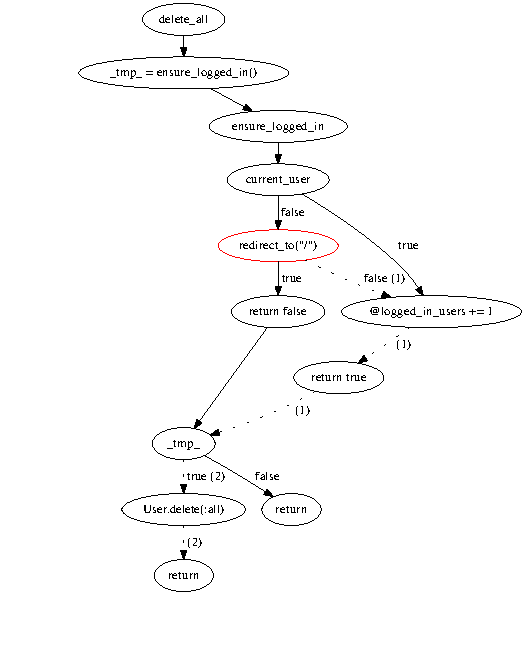
\includegraphics{figures/complex_ear_diagram.ps}
  \caption{Control Flow Graph for the code shown in
    Listing~\localref{code:false-positive}. The dotted lines are paths removed
    from the CFG by Step 3 of the EAR detection algorithm.}
  \locallabel{false-positive-cfg}
\end{figure*}


% \pagebreak[2]
\noindent\textbf{Step 3: Prune Infeasible Paths}\\
Looking for all paths from the \texttt{redirect\_to} method to the program
exit point might lead to false positives due to infeasible paths. Consider
the example in Listing~\localref{code:false-positive}. There are no EARs in this
code. The \texttt{redirect\_to} on Line~4 will always return \texttt{true},
thus, \texttt{return false} (also on Line~4) will execute as well. Because
of this, \texttt{ensure\_logged\_in} will always return \texttt{false}
after performing a redirect. As a result, the call to
\texttt{ensure\_logged\_in} on Line~11 will always return \texttt{false},
and the \texttt{return} on Line~12 will always occur.

The CFG for the code in Listing~\localref{code:false-positive} is shown in
Figure~\localref{false-positive-cfg}. With no additional processing, we would
incorrectly report the path from \texttt{redirect\_to} on Line~4 to the
statement in Line~6. Moreover, we would also report an EAR because of the
path from the redirect to the \texttt{User.delete} on Line~13. The first
path is denoted as (1) in Figure~\localref{false-positive-cfg}, the second path
as (2).

To prune infeasible paths in the CFG, we explore all paths that follow an
interesting method. If \emph{all} paths following an interesting method
call return the same Boolean value, we propagate this Boolean constant to
all the call sites of this method. Then, we recursively continue constant
value propagation at all the call sites, pruning infeasible paths
everywhere after the interesting method is called. We iteratively continue
this process throughout the CFG; whenever we find a constant return value,
we propagate this return value to all call sites.

Figure~\localref{false-positive-cfg} shows the results of performing our pruning
process on the CFG of Listing~\localref{code:false-positive}. Initially, all
paths after the \texttt{redirect\_to} in \texttt{ensure\_logged\_in} do not
return the same Boolean, so we cannot conclude anything about the return
value of \texttt{ensure\_logged\_in}. However, \texttt{redirect\_to} always
returns \texttt{true}. Therefore, we perform constant value propagation on
the return value of \texttt{redirect\_to}, which is used in a branch. As a
consequence, we can prune all of the paths that result from the
\texttt{false} branch. The edges of this path are labeled with (1) in
Figure~\localref{false-positive-cfg}. Now, all paths from \texttt{redirect\_to}
return \texttt{false}, which means that \texttt{ensure\_logged\_in} will
always return \texttt{false} after a redirect. We now perform constant
value propagation at all the call sites of \texttt{ensure\_logged\_in},
removing all the paths labeled with (2). At this point, there is nothing
more to be pruned, so we stop. It can be seen that there is no path from
\texttt{redirect\_to} to state-changing code (defined in the next step)
along the solid lines. \\

\noindent\textbf{Step 4: Detecting EARs}\\
Once the CFG of the controller has been simplified and interesting method
information has been extracted, we perform EAR detection. This is a
fairly simple process; we traverse the CFG of every method to see if
potentially problematic code can be executed after a call to an interesting method. We conservatively define such code
as any statement that could possibly modify the program state,
excluding statements that alter the control flow. This excludes
\texttt{return} and branches, but includes assignment and method
calls. As a special case, we also disregard all operations that set
the \texttt{flash} or \texttt{session} array variable. These arrays
are used in the former case to set a message to be displayed on the
destination page, and in the latter case to store some information in
the user's session. These calls are disregarded because they do no
affect the state of the web application and are frequently called
after redirection. We report as a potential EAR each method that
executes potentially problematic code between the invocation of an interesting method and its
return statements. 
\\

\noindent\textbf{Step 5: Distinguishing Between Benign and Vulnerable EARs}\\
We also introduce a heuristic to identify vulnerable EARs. This
heuristic looks for paths from an interesting method to a function that
modifies the database. If one is found, the EAR is marked as
vulnerable. We used the Rails documentation to determine the 16
functions that modify the database. Of course, this list can be easily extended.
This process is not sound, because we perform no type analysis, and
look only at the method names being called. Moreover, we do not
analyze the models, only looking for this specific list. Despite these
limitations, our results (Section~\localref{effectiveness}) show that this
heuristic is still a good indicator of potentially vulnerable
EARs that deserve the developer's attention.

\subsection{Limitations}
\locallabel{limitations}
The white-box EAR detector is limited to analyzing Ruby on Rails
applications, although the detection algorithm can be extended to any
programming language and web framework. Detection is neither sound nor
complete. False negatives can occur when a Rails application uses Ruby's
dynamic features such as \texttt{eval} or \texttt{send} to execute a
redirect. While such dynamic features are used extensively in the Ruby on
Rails framework itself, they are rarely used by web applications written in
Rails. Of the 3,457,512 method calls in controllers that we tested our tool
on, there were 428 (0.012\%) \texttt{eval} method calls and 2,426 (0.07\%)
\texttt{send} method calls, which shows how infrequently these are used in
Rails web applications.

The white-box tool can report two types of false positives: false
EARs, that is, the tool reports an EAR although no code can be
executed after a redirect, or false vulnerable EARs, where the tool
mistakes a benign EAR as vulnerable.

False EARs can occur for several reasons. One reason is that the path from
the redirect function to the code execution that we found is infeasible. A
typical example is when the redirect call and the code execution occur in
opposite branches. The branch conditions for these are mutually exclusive,
so there can never be a path from the redirect call to the code execution.
Examples of this type of false positive are discussed in
Section~\localref{effectiveness}, and these could be mitigated by introducing
better path sensitivity.

\begin{table}[tb]
  \centering
  \begin{tabular}{lr}
    Type of EAR reported & Number reported \\
    \hline
    Benign & 3,089 \\
    Vulnerable & 855 \\
    Total & 3,944 \\
    \hline
    \hline
    Total Projects & 18,127 \\
    Any EAR & 1,173 \\
    Only Benign & 830 \\
    At least one vulnerable EAR & 343 \\
    \hline
  \end{tabular}
  \caption{Results of running the white-box detector against Ruby on
    Rails applications, 6.5\% of which contained an EAR flaw. 2.9\% of
    the projects had an EAR classified as vulnerable.}
  \locallabel{white-box-results}
\end{table}



False vulnerable EARs are a problem caused by the heuristic that we use.
The biggest issue is that we simply look for method calls that have
the same name as method calls that update/change the database.
However, we do not perform any type analysis to determine the
\emph{object} that the method is called on. Thus, methods such as
\texttt{delete} on a hash table will trigger a false vulnerable EAR,
since \texttt{delete} is also a method of the database object.
Improved heuristics could be developed, for instance, that include the
type of the object the method is being invoked on.

Despite these limitations, our experiments demonstrate that the tool
works very well in practice. In addition, Ruby on Rails controllers
are typically very small, as most application logic is present in the
models. Thus, our tool works very well on these types of controllers.
We
provide\footnote{\url{https://github.com/adamdoupe/find\_ear\_rails}}
our tool to the community at large, so that others may use it to
detect EARs in their code.


\section{Results}
\locallabel{results}

We used our EAR detection tool to find real-world EARs in open-source Ruby
on Rails web applications. First, we downloaded 59,255 open-source projects
from GitHub~\cite{github} that were designated as Ruby projects and that
were not a fork of another project. We identified 18,127 of the downloaded
Ruby projects that had an \texttt{app/controllers} folder, indicating a
Ruby on Rails application.

Table~\localref{white-box-results} summarizes the results. In total, we
found 3,944 EAR instances in 1,173 projects. 855 of these EARs,
present in 343 projects, were classified as vulnerable by our system. This means
that 6.5\% of Rails applications we tested contained at least one EAR,
and 29.3\% of the applications containing EARs had an EAR classified as
vulnerable.

Of the 1,173 projects that contained at least one EAR, we notified those
project owners that had emails listed in their GitHub profile, for a total
of 624. Of these project owners, 107 responded to our email. Half of the
respondents, 49, confirmed the EARs we reported. 26 other respondents told
us that the GitHub project was no longer being maintained or was a
demo/toy. Three respondents pointed out false positives, which we
confirmed, while 6 of the project owners said that there were not going to
fix the EAR because there was no security compromise. The rest of the
responses thanked us for the report but did not offer a confirmation of the
reported EAR. 

\subsection{Detection Effectiveness}
\locallabel{effectiveness}
\begin{table}[tb]
  \centering
  \begin{tabular}{lr}
    Classification after manual analysis & Number \\
    \hline
    True Vulnerable EARs  & 485 \\
    Benign EARs  & 325 \\
    No EARs (False Positives)  & 45 \\
    \hline
  \end{tabular}
  \caption[Results of manually inspecting all vulnerable EARs.]{Results of manually inspecting the 855 vulnerable EARs
    reported by our white-box tool. 40.1\% were benign, and 5.3\% were
    not EARs.}
  \locallabel{white-box-analysis}
\end{table}


To determine the effectiveness of our tool, we manually inspected all
855 vulnerable EARs. The results are shown in
Table~\localref{white-box-analysis}. We manually verified that 485, or
59.9\%, were true positives. Many of these were caused by ad-hoc
authorization checks, where the developer simply introduced a redirect
when the check failed. Some examples of security violations 
were allowing non-administrators access to administrator
functionality, allowing modifications to items not belonging to the
current user, and being able to sign up for a conference even though
it was full.

{\ssp
\begin{lstlisting}[language=Ruby, caption={[True positive EAR vulnerability example.]True positive Execution
  After Redirect vulnerability in Ruby on Rails.},
    label=\currentprefix:code:interesting-ear, float]
class BanksController < ApplicationController 
  def redirect_to_login
    redirect_to("/login") and return
  end

  def create
    if not current_user.is_admin?  
      redirect_to_login() and return
    end  
    @bank = Bank.create(params[:bank])
  end  
end 
\end{lstlisting}
}


Listing~\localref{code:interesting-ear} shows
an interesting example adapted from a real EAR where the redirect is followed by \texttt{and return} (Line~3),
however, due to Ruby's semantics, this code contains an EAR. In Ruby,
a \texttt{return} with no arguments returns \texttt{false}\footnote{Technically
  \texttt{nil}, but \texttt{nil} and \texttt{false} are equivalent for
  Boolean comparisons.}, 
thus, \texttt{redirect\_to\_login} will always return \texttt{false} (because of
the ``no argument'' \texttt{return} call on Line~3). The result is that the
\texttt{return} on Line~8 will never be executed, because
\texttt{redirect\_to\_login} will always return \texttt{false}, and
the short-circuit logic of \texttt{and} will cause Line~10 to be
executed. This example shows that our tool discovers non-obvious EARs.

For vulnerable EARs, we consider two different types
of false positives: false \emph{vulnerable} EARs, which are benign EARs
mistakenly reported as vulnerable, and false EARs (false positives).

As shown in Table~\localref{white-box-analysis}, the white-box tool
generated 45 false EARs, for a false positive rate of 5.3\%. These
false positives came from two main categories. About half of the false
positives were due to  impossible paths from the redirect methods to
some code. An example of this is when a redirect method was called at
the end of a branch that checked that the request was an HTTP GET,
while the code executed after a redirect was in a branch that checked
that the request was an HTTP POST. These two conditions are mutually
exclusive, thus, this path is impossible. The other half of false
positives were due to local variables that had the same name as a
redirect method. The parsing library, RIL, mistakenly identified the
local variable access as a method call to a redirect method. We are
currently looking into fixing this issue in RIL, which will almost
halve our false positive rate.

While our false EAR rate was only 5.5\%, our vulnerable EAR detection
heuristic had a higher false detection rate of 40.1\%. The biggest culprit
for false vulnerable EARs (72.9\% of the instances) was due to no feasible
path from the redirect to the method that changed the state of the
database. For instance, the redirect method occurred in a branch that was
taken only when a certain object was \texttt{nil}\footnote{\texttt{nil} is
  Ruby's \texttt{null}.}. Later, the database method was called on this
object. Thus, when the redirect happens, the object will be \texttt{nil}.
Because of the presence of an EAR flaw, execution will continue and reach
the database access method. However, since the object is \texttt{nil}, the
database will not be affected. Because our heuristics cannot detect the
fact that, after the redirect, the database function will always be called
with a \texttt{nil} object, we report a vulnerability. The other common
false vulnerable EAR were instances where the redirect method was called
before code was executed, however, it was clear that the developer was
fully aware of the redirect semantics and intended for the code to be
executed.

We also checked that the false EAR rate did not differ significantly among
the benign EARs by manually inspecting 200 random EARs reported as benign.
We saw 13 false EARs in the manual inspection, for a false positive rate of
6.5\%. Thus, the total false positive rate among the instances we manually
inspected is 5.5\%. We also did not see any vulnerable EARs among the
benign EARs, thus, we did not see any false negative vulnerable EARs in our
experiments.

From our results, we can conclude that we detect EARs well. However,
it is more difficult to distinguish between benign and vulnerable EARs.
Classification could be improved by using a better heuristic to detect
intended redirects. However, even though certain EARs might not be
vulnerable at the moment, they are still programming errors that
should be fixed. This is confirmed by the responses that we received
from developers who were grateful for error reports even though they
are not exploitable at the moment. Also, our tool reports one true
vulnerability for every benign EAR mistakenly classified as
vulnerable. This is well in line with the precision of previous static
analysis
tools~\cite{jovanovic06:pixy-short,huang04:securing,livshits05:java-static}.

\subsection{Performance}

To evaluate the performance of our tool, we measured the running time
against the 18,127 Ruby on Rails applications. We ran our experiments on an
Intel Core i7 with 12 gigabytes of RAM. Our algorithm scales linearly with
the size of the CFG and is fast; no project took longer than 2.5 seconds
even with the largest CFG size of 40,217 statements.

\section{Prevention}
\locallabel{prevention}

The old adage ``an ounce of prevention is worth a pound of cure'' is true
in software. Boehm showed that the later in an application's life-cycle
bugs are caught, the more expensive they are to fix~\cite{boehm81:see}.
Thus, preventing certain types of bugs from even being introduced is
attractive from both an economic standpoint, and a security perspective. Our
recommendation to web frameworks, therefore, is to make Execution After
Redirect vulnerabilities impossible to occur, by having every invocation of
the redirect method halt execution, which we call halt-on-redirect
behavior.

As we have shown in Section~\localref{framework-analysis}, some frameworks
have already either adopted the approach of making EARs impossible, or
their approach to generating HTTP responses makes EARs highly
unlikely. For existing frameworks that wish to decrease the chance of
EARs being introduced, such draconian measures may not be acceptable
because they break backward-compatibility. Our suggestion in these
cases is to make an application-wide setting to enable
halt-on-redirect behavior, along with an argument to the redirect
function to halt execution after the redirect. Of course, we suggest
making halt-on-redirect the default behavior, however each framework
will have to properly balance security and backward-compatibility.

To improve the security of Ruby on Rails, we are in discussions with the
Rails development team about our proposed change. The difficulty with
implementing halt-on-redirect behavior in Rails is that there are no
\texttt{goto}s, and Rails applications run in a single-threaded context.
This limits the two obvious forms of implementing halt-on-redirect: we
cannot use a go\-to or language equivalent statement to jump from the end
of the \texttt{redirect\_to} method to the code after the controller is
called. Moreover, we also cannot, at the end of the \texttt{redirect\_to}
method, send the HTTP response and cause the current thread to stop
execution. PHP frameworks can use the \texttt{exit} function to implement
halt-on-redirect behavior, because each request spawns a new PHP process.

Our proposed solution is to throw a new type of exception,
\texttt{RedirectOccuredException}, at the end of the
\texttt{redirect\_to} body. In the Ruby on Rails framework core, where
the controller is called, there is a catch block for this exception.
While this will prevent almost all EARs, there is a possibility for
code to be executed in an \texttt{ensure} block, Ruby's equivalent of
a ``finally'' block. Code in this block will be executed regardless of a
redirect. However, we believe this is semantically in line with the
way the language should work: ensure blocks will always be executed,
no matter what happens, and this is clear to the programmer via the
language's semantics.


\section{Conclusions}
\locallabel{conclusion}

We have described a new type of vulnerability, Execution After Redirect,
and developed a novel static analysis tool to effectively find EARs. We
showed that EARs are difficult to differentiate between benign and
vulnerable. This difficulty is due to vulnerable EARs violating the
specific logic of the web application. Better understanding of the
application's logic should help differentiate vulnerable and benign EARs
and it will be the focus of future work.

%% \subsection*{Acknowledgments}
%% This work was also partially supported by the ONR under grant N000140911042
%% and by the National Science Foundation (NSF) under grants CNS-0820907,
%% CNS-0905537, and CNS-0716095.

%% \bibliographystyle{acm}
%% \bibliography{biblio,other}

